\documentclass[10pt]{article}
% \usepackage[utf8]{inputenc}
\usepackage[letterpaper, margin=1in, headheight=105pt]{geometry}
\usepackage{subcaption}
\usepackage{enumerate}
\usepackage{mathtools}
\usepackage{listings}
\usepackage{fancyhdr}
\usepackage{graphicx}
\usepackage{amsmath}
\usepackage{amssymb}
\usepackage{caption}
\usepackage{xparse}
\usepackage{amsthm}
\usepackage{float}
\usepackage[dvipsnames]{xcolor}
\usepackage[colorlinks=true,linkcolor=red,anchorcolor=yellow,
citecolor=green,urlcolor=cyan,filecolor=brown,menucolor=brown]{hyperref}
% \usepackage{calligra}
% \usepackage{titlesec} % screw the fancyhdr
% \usepackage{comment}
\usepackage[numbered,framed]{matlab-prettifier}
% /usr/share/texlive incomplete
% /usr/local/texlive complete 2017

\lstset{language=python,basicstyle=\ttfamily,keywordstyle=\color{blue}\ttfamily,
stringstyle=\color{red}\ttfamily,commentstyle=\color{green}\ttfamily,morecomment=[l][\color{magenta}]{\#}}

\geometry{letterpaper}
\pagestyle{fancy}
% \lhead{\href{https://mcommunity.umich.edu/\#search:yugtmath}{UMID: 97318705}}
% \rhead{\href{mailto:yugtmath@umich.edu}{yugtmath@umich.edu}}
% \chead{\href{http://www-personal.umich.edu/~yugtmath}{\calligra{Guangting Yu}}}
\lfoot{\href{https://umich.instructure.com/courses/173857}{\textbf{University of Michigan, Ann Arbor}}}
\rfoot{\href{https://github.com/yugt/ComupterVision}{\textbf{EECS 442 Computer Vision, F2017}}}

% \renewcommand{\thesection}{HW \arabic{section}}
\renewcommand{\thesubsection}{\arabic{subsection}}
% \titleformat{\subsection}{\normalfont\large\bfseries}{Problem \thesubsection:}{5pt}{}

\lstset{xleftmargin=.05\textwidth, xrightmargin=0.02\textwidth}
\title{EECS 442 Computer Vision}
% \author{\calligra{Guangting Yu}\textrm{,}\hspace{5pt} \texttt{yugtmath}}
\author{Guangting Yu\textrm{,}\hspace{5pt} \texttt{yugtmath}}
\date{\today}

\begin{document}
\maketitle
\tableofcontents
\newpage
\listoffigures
\newpage

%!TEX root = ../main.tex
\section{Homework \thesection}


\subsection{Fitting Curves with Linear Least Squares}
We discussed the least-square formulation for a slope-intercept model of a line during lecture.
\begin{equation}\label{linearregression}
E(m, b)=\sum_{i=1}^{n}[y_i-mx_i-b]^2
\end{equation}
And we also talked about fitting a quadratic curve using LLS.
Now, assume you got some sample points from some experiments, i.e., \href{./hw1/problem1/hw1_p1.mat}{\texttt{hw1\_p1.mat}} in the problem1 folder.

\begin{enumerate}
	\item Say you want to fit the data to a cubic curve.
	Write down the least squares formulation (in a form similar to Eq.\ref{linearregression}) as well as the matrix formulation of it.
	Explain why this problem could be solved by using Linear Least Squares despite the fact that the curve is non-linear.
	\item Implement the solution of the LLS problem you wrote in (1).
	Report resulting coefficient values and a plot of the fit;
	include your code verbatim in your pdf submission.
	The file named \href{./hw1/problem1/viz_curve.m}{\texttt{viz\_curve.m}} will plot the curves for you.
	Increase the order of curves, such as 4,5 and 6, and report their resulting plots as well.
	\item Does the curve with higher orders fit the data better?
	Explain what you observe.
\end{enumerate}


\subsubsection{Cubic model}
The least squares formulation of cubic curves is
\begin{equation}
E(b_3,b_2,b_1,b_0)=\sum_{i=1}^{n}\left[y_i-\left(b_3 x_i^3 + b_2 x_i^2 + b_1 x_i + b_0 \right)\right]^2.
\end{equation}
Linear Least Square does not mean the curve needs to be linear.
Here, linear means that the response should be a linear combination of predictors.
As long as the predictors are linearly independent, we can always use the Linear Least Square method.
The key point is to define a proper set of predictors.
From linear algebra, we know that polynomials with different degrees are independent.
Since cubic curves have degree at most 3, the set of linearly independent polynomials has dimension 4.
For simplicity, we do not require the basis to be orthogonal.
Instead, we take the simpliest basis: \(x^3, x^2, x, 1\).
The Least Square method is to determine the linear combination that minimize the sum of square errors.
If written in matrix form,
\begin{equation}
\begin{bmatrix}
y_1 \\ y_2 \\ \vdots \\ y_n
\end{bmatrix}
=
\begin{bmatrix}
x_1^3 & x_1^2 & x_1 & 1 \\
x_2^3 & x_2^2 & x_2 & 1 \\
\vdots & \vdots & \vdots & \vdots \\
x_n^3 & x_n^2 & x_n & 1
\end{bmatrix}
\begin{bmatrix}
b_3 \\ b_2 \\ b_1 \\ b_0
\end{bmatrix}
+
\begin{bmatrix}
e_3 \\ e_2 \\ e_1 \\ e_0
\end{bmatrix},
\end{equation}
or equivalently,
\begin{equation}
Y=Xb+e.
\end{equation}
And the sum of square error is
\begin{equation}
E(b_3,b_2,b_1,b_0)=e^Te
\end{equation}
According to the result from multilinear regression, the best \(b\) that minimize the square error is
\begin{equation}
b=\left(X^T X\right)^{-1}X^TY
\end{equation}

\subsubsection{Implementation}
The implementation is very short.
And I tried the increased order of curves, up to order 7.
The code and plots (Figure \ref{fig:1}) are listed below.
\begin{lstlisting}[style=Matlab-editor]
x=[X.^3 X.^2 X.^1 X.^0]
C3=inv(x'*x)*x'*Y
x=[X.^4 X.^3 X.^2 X.^1 X.^0]
C4=inv(x'*x)*x'*Y
x=[X.^5 X.^4 X.^3 X.^2 X.^1 X.^0]
C5=inv(x'*x)*x'*Y
x=[X.^6 X.^5 X.^4 X.^3 X.^2 X.^1 X.^0]
C6=inv(x'*x)*x'*Y
x=[X.^7 X.^6 X.^5 X.^4 X.^3 X.^2 X.^1 X.^0]
C7=inv(x'*x)*x'*Y
viz_curve(C3,X,Y)
viz_curve(C4,X,Y)
viz_curve(C5,X,Y)
viz_curve(C6,X,Y)
viz_curve(C7,X,Y)
\end{lstlisting}

The coefficients are
\begin{equation}
\begin{bmatrix}
b_3 \\ b_2 \\ b_1 \\ b_0
\end{bmatrix}
=
\begin{bmatrix}
	-0.00866565736949468\\
	-0.205773475198218\\
	2.34336989430312\\
	1.26227984182860
\end{bmatrix}
\end{equation}


\begin{figure}[htbp]
	\centering
	\begin{subfigure}[t]{0.5\textwidth}
		\centering
		\includegraphics[width=\textwidth]{hw1/problem1/f1.pdf}
		\caption{Order 3}\label{fig:1a}
	\end{subfigure}

	\begin{subfigure}[t]{0.42\textwidth}
		\centering
		\includegraphics[width=\textwidth]{hw1/problem1/f2.pdf}
		\caption{Order 4}\label{fig:1b}
	\end{subfigure}
	\quad
	\begin{subfigure}[t]{0.42\textwidth}
		\centering
		\includegraphics[width=\textwidth]{hw1/problem1/f3.pdf}
		\caption{Order 5}\label{fig:1c}
	\end{subfigure}
	\begin{subfigure}[t]{0.42\textwidth}
		\centering
		\includegraphics[width=\textwidth]{hw1/problem1/f4.pdf}
		\caption{Order 6}\label{fig:1d}
	\end{subfigure}
	\quad
	\begin{subfigure}[t]{0.42\textwidth}
		\centering
		\includegraphics[width=\textwidth]{hw1/problem1/f5.pdf}
		\caption{Order 7}\label{fig:1e}
	\end{subfigure}
	\caption{Linear Least Square fit on models of different orders}\label{fig:1}
\end{figure}



\subsubsection{Observation and discussion}
In general, \emph{if the sum of square error is the rubric to evaluate the fitness, then the higher the interpolation order, the smaller the sum of square error, which indicates the better fitness.}
This is because the higher order interpolation has more coefficients to minimize the errors at each \(x_i\).
The extreme case is the number of coefficients equals to the number of data points, which leads to perfect interpolation and no errors.

However, it seems from Figure \ref{fig:1a} that the cubic curve follows the trend of the points quite well.
In comparison, when the order increases, the trend becomes wired, although the curve seems to be closer to every point.
This shows that curve with higher orders may not fit the data better, which may be called as \emph{overfit}.
And when the order reaches 7, MATLAB shows the warning ``Matrix is close to singular or badly scaled. Results may be inaccurate.'' and provide the condition number of \(X^T X\) is 8.4867e+17, which means it is nearly singular.
Furthermore, the round-off error due to the precision limit of MATLAB will cause a relatively large error.



\subsection{Lambertian Model}
Recall the Lambertian model of reflectance:
\begin{equation}\label{lambertian}
R(x) = \rho l(x)^T n(x)
\end{equation}
\begin{enumerate}
	\item There are two people standing at location A and B.
	Who will observe stronger reflection at point x? Why?
	\item Tell one drawback of Lambertian model and name a specific object in the real world whose reflectance is not well modeled by the Lambertian model.
\end{enumerate}

\subsubsection{Reflection intensity}
Since the reflection intensity only depends on \(\rho\) and \(x\), it is the same for both observers.
% Recall that any reflected light intersecting an image plane, by way of a camera projection function \(P\), would induce a perfect image:
% \begin{equation}\label{perfectimage}
% \mathcal{I}(u)=P(R(x))
% \end{equation}
% We can observe that for a fixed \(R(x)\), the projection on the B's plane is shorter than the one on A's plane.
% This means that the intensity of refection observed by B is greater than the one by A.
% So B observes a stronger reflection.

\subsubsection{Drawback of Lambertian model}
The practical drawback of Lambertian model is that it is too simple (sometimes naive).
It only gives the intensity of reflection as a scale.
It cannot describe the easiest case -- mirror reflection -- in physics.

Mathematically, this model will fail when the normal vection \(n(x)\) is not defined.
In 3 dimensional case, the normal vector can be obtained by the cross product of two linearly independent tangent vector, and the tangent vectors can be defined by the partial derivatives.
So if the surface is not differentiable, the Lambertian model will fail.
For example, the edge of a knife, the point of a needle or the boundary of a Koch snowflake.




\subsection{Bayer Demosaicking}
To digitalize a perfect color image, we overlay the Bayer pattern filter on top of the photo sensors to accept RGB separately.
We could call this process mosaicking.
Assume that you've got a digital image filtered by the Bayer pattern and want to demosaic it, i.e., reconstruct the original color image.
One of the common ways to do this is to use bilinear interpolation.
For a green pixel, two red neighbors can be interpolated to yield the red value and two blue neighbors can be interpolated to yield the blue value, and similar for red or blue pixels.
The only difference is that for red or blue pixels you need to consider 4 neighbors instead of 2.

In Matlab, the function \texttt{demosaic} actually does this job, but now you need to implement this function by your own.
Pick any color image you like and use bayer filter.m to generate a Bayer encoded image.
Implement the demosaicking algorithm in \href{./hw1/problem3/mydemosaic.m}{\texttt{mydemosaic.m}}.
Report the original image, filtered image and reconstructed image; include your \href{./hw1/problem3/mydemosaic.m}{\texttt{mydemosaic.m}} verbatim in your pdf submission with brief explanation.
Submit your code together with your report.

\lstinputlisting[style=Matlab-editor]{./hw1/problem3/mydemosaic.m}

The code listed above with some comments is the implementation of \href{./hw1/problem3/mydemosaic.m}{\texttt{mydemosaic.m}}.
Most of the code (loops and if-else cases) deals with the boundary conditions, since MATLAB will report overflowed index on the boundary if we forget to check.
The result is quite satisfying.
I use an image that I took personally at the Palace of Fine Arts in San Francisco.
Three standard size photos were taken and stinched together to create Figure \ref{fig:2}.



\begin{figure}[htbp]
	\centering
	\begin{subfigure}[t]{\textwidth}
	    \centering
		\includegraphics[width=0.95\textwidth]{hw1/problem3/homepage.jpg}
		\caption{Original image}\label{fig:2a}
	\end{subfigure}
	\begin{subfigure}[t]{\textwidth}
	    \centering
		\includegraphics[width=0.95\textwidth]{hw1/problem3/gray.png}
        \caption{Filtered image}\label{fig:2b}
	\end{subfigure}
	\begin{subfigure}[t]{\textwidth}
	    \centering
		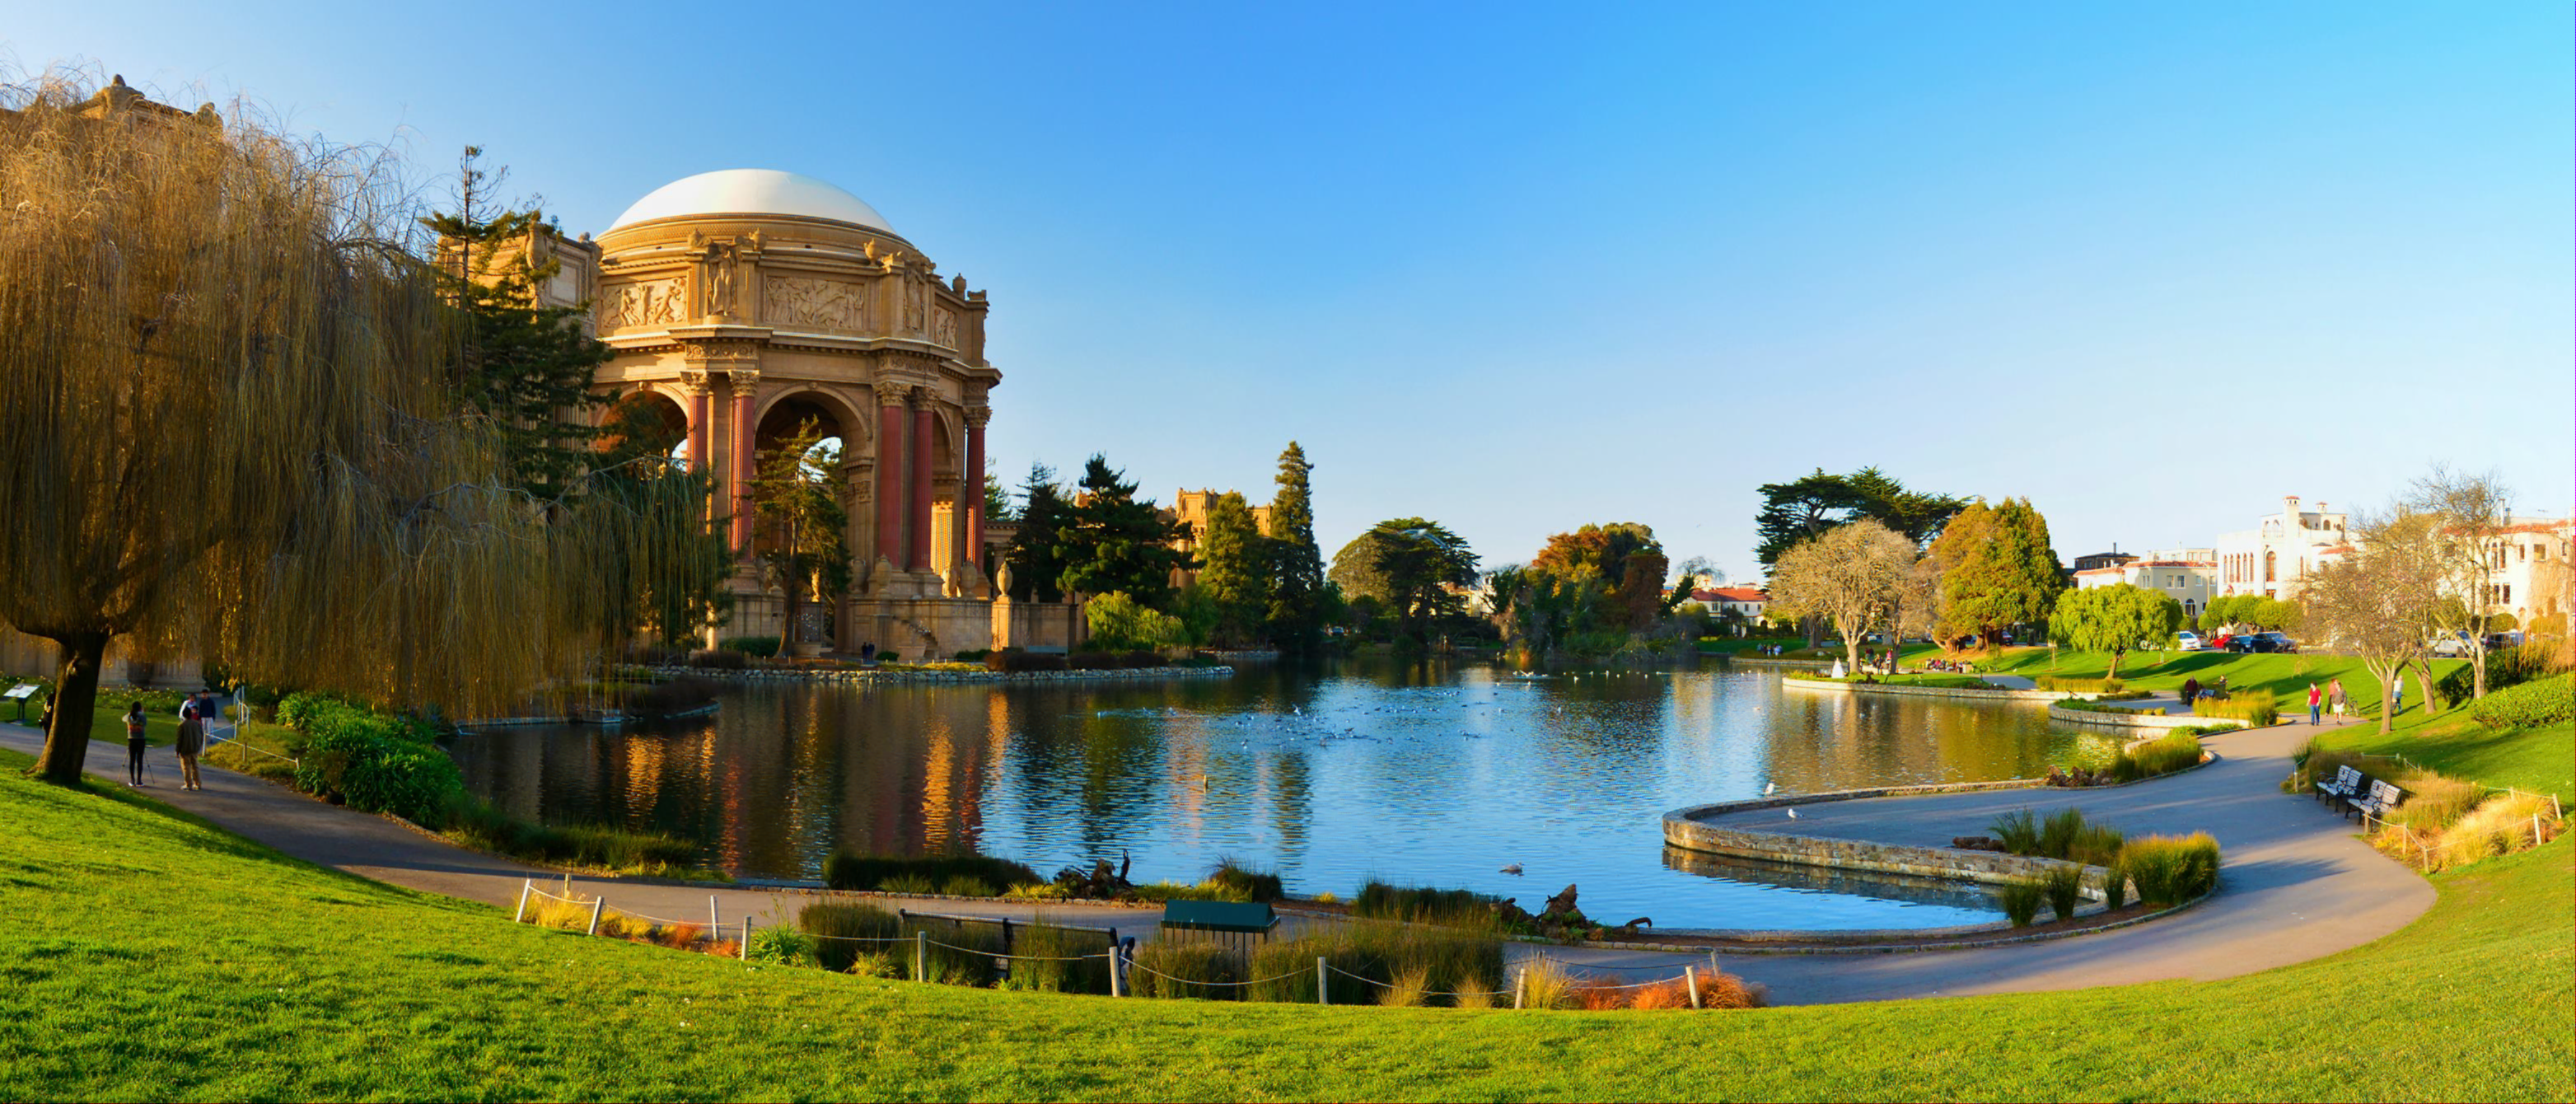
\includegraphics[width=0.95\textwidth]{hw1/problem3/reconstructed.png}
		\caption{Reconstructed image}\label{fig:2c}
	\end{subfigure}
	\caption{Palace of Fine Arts, San Francisco \copyright}\label{fig:2}
\end{figure}


\subsection{Potts Model on Color Images}
Recall the Potts Model that was discussed as a mechanism for modeling piecewise constant images and regularizing region boundaries.
It was shown in the class that how to implement Potts model with loops.
Now you need to implement the Potts model using ideas of \textbf{Spatial Range Map} operators.
The images we are considering here are discrete color images with RGB three channels and for every channel values range from 0 to 255.
You should complete the function \href{./hw1/problem4/potts.m}{\texttt{potts.m}} to return the \(E(I)\) for the given image.
The provided code potts \href{./hw1/problem4/potts_load.m}{\texttt{potts\_load.m}} will load in the images, call \href{./hw1/problem4/potts.m}{\texttt{potts.m}} and display the results for you.
For all code, use \(\beta=1\).
Run and report output figures of \href{./hw1/problem4/potts_load.m}{\texttt{potts\_load.m}}; include your \href{./hw1/problem4/potts.m}{\texttt{potts.m}} verbatim in your pdf submission with brief explanation.
Submit your code together with your report.

\emph{Hint}: the input image is in the format of uint8 and you might need to turn it to double to yield correct answer.


\lstinputlisting[style=Matlab-editor]{./hw1/problem4/potts.m}

In comparison with the previous problem this function is suprisingly short, where there are only 4 lines of effective code (line 12-15).
This is because we use the select row and select column functions to avoid the loop.
The output results are shown in Figure \ref{fig:3}.
The more complex the image is, the larger the entropy is.
Obviously, \ref{fig:3b} has more patterns than \ref{fig:3a}, so it has larger \(E\) .

\begin{figure}[htbp]
	\centering
	\begin{subfigure}[t]{\textwidth}
	    \centering
		\includegraphics[width=0.8\textwidth]{hw1/problem4/i1.pdf}
		\caption{\texttt{I1}, \(E=36\)}\label{fig:3a}
	\end{subfigure}
	\begin{subfigure}[t]{\textwidth}
	    \centering
		\includegraphics[width=0.8\textwidth]{hw1/problem4/i2.pdf}
		\caption{\texttt{I2}, \(E=42\)}\label{fig:3b}
	\end{subfigure}
	\caption{Potts Model of Color Images}\label{fig:3}
\end{figure}
%!TEX root = ../main.tex
\section{Homework \thesection}

\subsection{Domain Operations}
Recall domain operations and geometric transformations discussed in the lecture.
\begin{enumerate}
\item Why do we use homogeneous coordinates?
\item In the 2D rigid transformation matrix
		\[ \begin{pmatrix}
		R & t \\ 0 & 1
		\end{pmatrix}, \]
		rotation is centered at the origin.
		Sometimes we need to rotate a point around another point instead of the origin.
		Assume that	there are two points \(o=(3,5)\) and \(p=(4,2)\) in the 2D plane.
		Write down the transformation matrix \(T\) that rotates \(p\) around \(o\) by \(45^\circ\) clockwise.
\item Implement a similarity transform in Matlab:
		\[T=\begin{pmatrix}
		\frac{\sqrt{3}}{3} & -\frac{1}{3} & 30 \\
		\frac{1}{3} & \frac{\sqrt{3}}{3} & 40 \\
		0 & 0 & 1
		\end{pmatrix}.
		\]
		It's recommended to read through \href{./hw2/2DGeometrixTransformationRecipe.pdf}{\texttt{2D Geometric Transformation Recipe}} before you start coding, especially if you are not very clear how you're going to do this.
		That doc includes the instructions and tips of implementation, which may save you the time to finish this task.
		Choose any image you like as the input image.
		For simplicity, turn the image into gray-scale if it is not.
		Report the original and the output image; include your verbatim in your pdf submission with brief comments.
		Submit your code together with your report.
\end{enumerate}

\subsubsection{Homogeneous coordinates}
Homogeneous coordinates is an extension of Cartesian coordinate (rectangular coordinate).
With this coordinate system, we can write the transformation in the form of matrix multiplication.
Cartesian coordinate can also reach this target, but with restricts.
For example, the projective transformation cannot be described in Cartesian coordinate, but it can be expressed in homogeneous coordinate.\\
Also, it has the property of linearity.
This makes the combination and addition easier than curvilinear coordinates such as spherical or cylindrical coordinates.\\
Last but not the least, homogeneous coordinate is complete in the field of rational numbers \(\mathbb{Q}\), while spherical and cylindrical coordinates always need irrational numbers since \(\pi\) is involved.


\subsubsection{Rotation centered at a non-origin point}
Assume the center of rotation is \((x_0, y_0, 1)^T\).
Then, we can first shift the center of rotation to the origin, then apply the normal rotation, and shift back.
Thus,
\[ \begin{bmatrix}x'\\ y'\\ 1 \end{bmatrix}=R\left(\begin{bmatrix}x\\ y\\ 1 \end{bmatrix}-\begin{bmatrix}x_0\\ y_0\\ 1 \end{bmatrix}\right)+\begin{bmatrix}x_0\\ y_0\\ 1 \end{bmatrix}. \]
Apply the normal rotation matrix and calculate the product,
\[ \begin{bmatrix}x'\\ y'\\ 1 \end{bmatrix}=\begin{bmatrix} \cos\theta & -\sin\theta & 0 \\ \sin\theta & \cos\theta & 0 \\ 0 & 0 & 1 \end{bmatrix}\begin{bmatrix} x-x_0 \\ y-y_0 \\ 0 \end{bmatrix}+\begin{bmatrix}x_0\\ y_0\\ 1 \end{bmatrix}=\begin{bmatrix} x\cos\theta-y\sin\theta+x_0(1-\cos\theta)+y_0\sin\theta \\ x\sin\theta+y\cos\theta-x_0\sin\theta+y_0(1-\cos\theta) \\ 1 \end{bmatrix}. \]
Writing it in the matrix form, we have
\[ \begin{bmatrix}x'\\ y'\\ 1 \end{bmatrix}=\begin{bmatrix} \cos\theta & -\sin\theta & x_0(1-\cos\theta)+y_0\sin\theta &  \\ \sin\theta & \cos\theta & -x_0\sin\theta+y_0(1-\cos\theta) \\ 0 & 0 & 1 \end{bmatrix}\begin{bmatrix}x\\ y\\ 1 \end{bmatrix}. \]
Plug in \((x_0,y_0)=(3,5)\) and \((x,y)=(4,2)\), and \(\theta=-45^\circ\), we obtained the transformation matrix
\[ T=\begin{bmatrix} \frac{\sqrt{2}}{2} & \frac{\sqrt{2}}{2} & 3-4\sqrt{2} \\ -\frac{\sqrt{2}}{2} & \frac{\sqrt{2}}{2} & 5-\sqrt{2} \\ 0 & 0 & 1 \end{bmatrix}. \]

\subsubsection{Similarity transformation}
The code for similarity transformation in natural (Cartesian) coordinate (right-hand rule) is listed below.
The transformation matrix is defined at line 2.
So the image seems to be rotated \(30^\circ\) counter-clockwise.
\lstinputlisting[style=Matlab-editor]{./hw2/problem1/similarity.m}
If we use the coordinate in Matlab style (left-hand rule), then the image will seem to be rotated \(30^\circ\) clockwise.
The code is nearly the same, except some coordinates are shifted.
\lstinputlisting[style=Matlab-editor]{./hw2/problem1/similarity_left_hand_coordinate.m}
The effect is shown in Figure \ref{fig:4}.
\begin{figure}[htbp]
	\centering
	\begin{subfigure}[t]{0.5\textwidth}
	    \centering
		\includegraphics[width=\textwidth]{hw2/problem1/Lenna.png}
		\caption{Original}\label{fig:4a}
	\end{subfigure}\\
	\begin{subfigure}[t]{0.4\textwidth}
	    \centering
		\includegraphics[width=\textwidth]{hw2/problem1/lena.png}
		\caption{Transformation in natural (Cartesian) coordinates (new homework)}\label{fig:4b}
	\end{subfigure}
	\qquad
	\begin{subfigure}[t]{0.4\textwidth}
	    \centering
		\includegraphics[width=\textwidth]{hw2/problem1/lenal.png}
		\caption{Transformation in Matlab style coordinates (old homework)}\label{fig:4c}
	\end{subfigure}
	\caption{Similarity Transformation}\label{fig:4}
\end{figure}



\newpage


\subsection{3D Structure Tensor}
The Harris operator we discussed at length in lecture computes and analyzes the eigenvalues of the 2D gradient structure tensor (you will implement it below in the third problem).
Let \(\lambda_1\) and \(\lambda_2\) denote the larger and smaller eigenvalues, respectively.
We set two criteria for selection feature points (the value of \(\lambda_2\) and the ratio \(\frac{\lambda_1\lambda_2}{\lambda_1+\lambda_2}\)) based on the analysis of the eigenvalues
(\textit{e.g.}, two small eigenvalues indicate a mostly absent gradient, one large and one small eigenvalue indicate an edge, and two large eigenvalues indicate a corner).\\
Now, consider a video parameterized over \((x,y,t)\in\mathbb{R}^3\).
The eigenvalues of the 3D gradient structure tensor will similarly stratify the pixels in the video into different types.
Let \(\{\lambda_1,\lambda_2,\lambda_3\}\) denote the three eigenvalues of this 3D structure tensor (sorted in decreasing order).
\begin{enumerate}
\item Derive the form of the 3D structure tensor from the SSD error function (for window \(W\)):
		\[ E(u,v,w)=\sum_{u,v,w\in W}\left[\mathcal{I}(x+u,y+v,t+w)-\mathcal{I}(x,y,t) \right]^2 \]
		Propose a criterion to extract ``3D corners''.
\item Answer the question ``What is a 3D corner?''.
		What is an example of a physical phenomenon that may give rise to three large eigenvalues?
		Remember this is space-time and not 3D space, such as that you would image with MRI, for example.
\end{enumerate}


\subsubsection{3D structure tensor derivation}
We apply Taylor's expansion up to first order on \(\mathcal{I}(x+u,y+v,t+w)\):
\[ \mathcal{I}(x+u,y+v,t+w)\approx\mathcal{I}(x,y,t)+\partial_x\mathcal{I}(x,y,t)\cdot u+\partial_y\mathcal{I}(x,y,t)\cdot v+\partial_t\mathcal{I}(x,y,t)\cdot w. \]
Then the SSD error function can be approximated by
\[ E(u,v,w)\approx\sum_{u,v,w\in W}\left(\partial_x\mathcal{I}(x,y,t)\cdot u+\partial_y\mathcal{I}(x,y,t)\cdot v+\partial_t\mathcal{I}(x,y,t)\cdot w\right)^2. \]
For simplicity, denote the partial derivatives as \(\mathcal{I}_x\coloneqq\partial_x\mathcal{I}(x,y,t)\), \(\mathcal{I}_t\coloneqq\partial_t\mathcal{I}(x,y,t)\), \(\mathcal{I}_t\coloneqq\partial_t\mathcal{I}(x,y,t)\), and we obtain the matrix form:
\[ E(u,v,w)\approx\begin{bmatrix} u & v & w \end{bmatrix} \underbrace{\begin{bmatrix} \sum_{u,v,w\in W}\mathcal{I}_x^2 & \sum_{u,v,w\in W}\mathcal{I}_x\mathcal{I}_y & \sum_{u,v,w\in W}\mathcal{I}_x\mathcal{I}_t \\ \sum_{u,v,w\in W}\mathcal{I}_x\mathcal{I}_y & \sum_{u,v,w\in W}\mathcal{I}_y^2 & \sum_{u,v,w\in W}\mathcal{I}_y\mathcal{I}_t \\ \sum_{u,v,w\in W}\mathcal{I}_x\mathcal{I}_t & \sum_{u,v,w\in W}\mathcal{I}_y\mathcal{I}_t & \sum_{u,v,w\in W}\mathcal{I}_t^2 \end{bmatrix}}_\text{3D structure tensor} \begin{bmatrix} u \\ v \\ w \end{bmatrix}. \]
And the matrix in the middle is the 3D structure tensor.
Since the 3D structure tensor is symmetric, its eigenvalues are real.
Furthermore, by construction, it is also positive semi-definite.
Using the analogy of 2D structure tensor, we can propose a criterion to select feature points:
\[ \frac{1}{\frac{1}{\lambda_1}+\frac{1}{\lambda_2}+\frac{1}{\lambda_3}}, \]
which mainly depends on the smallest eigenvalue \(\lambda_3\).
If \(\lambda_3\gg0\), then this value will be large, and will be detected as 3D corner.

\subsubsection{3D corner definition and example}
The 3D corner should be a moving 2D corner on \((x,y)\in\mathbb{R}^2\).
If the corner is static, then \(\mathcal{I}_t=0\), and thus \(\lambda_3=0\), which will not be selected by the criterion.
If the 2D structure is not a corner, then it already has a small eigenvalue, so no matter it is moving or not, it will not be selected as a 3D corner.
An example is a falling box in a static background.
The vertices of the box will be recognized as 3D corners.


\subsection{Local Image Features and Image Stitching}
We motivated and derived an initial local image feature point detector based on an eigendecomposition of the structure tensor.
We also demonstrated an application example of image stitching.
In this question, you will explore these topics further.
\begin{enumerate}
\item Implement the local structure tensor construction and eigendecomposition as described in class.
		This method is called Harris, but implement the simplified corner response measure based on the minimum eigenvalue of the structure tensor, as discussed in class.
		The source file to which you should add code is \href{./hw2/problem3/harris.m}{\texttt{harris.m}}.
		It includes a comment block indicating where you should fill in your code.
		The function should return \texttt{C} where every pixel contains the corner strength.
		This is a ``corner response image''.
		To test your code, you should run \href{./hw2/problem3/run_3_1.m}{\texttt{run\_3\_1.m}}, which will load a simple checkerboard image and execute your harris function on it.
		This will generate two images in figures and save them to disk.
		\href{./hw2/problem3/response_checkerboard.png}{\texttt{response\_checkerboard.png}} is the checkerboard response image (directly from harris) and \href{./hw2/problem3/detect_checkerboard.png}{\texttt{detect\_checkerboard.png}} is the actual corner detections.
		The detect script will run a non-maximal suppression routine and extract corner locations from the response image.\\
		Include two images as well as your code verbatim in the pdf report.
		Submit the \href{./hw2/problem3/harris.m}{\texttt{harris.m}} together with the report.
\item Run the \href{./hw2/problem3/run_3_2.m}{\texttt{run\_3\_2.m}} script; it will load an image of \href{./hw2/problem3/rings.png}{concentric rings} and generate a corner response image \href{./hw2/problem3/response_rings.png}{\texttt{response\_rings.png}}.
		Please discuss the response image explaining why it looks like it does.
		Specifically describe why there are so many responses yet there are no ``corners'' in the image, and why, even though, there are many responses, no full ring has a high corner response over the entire ring.
		Include the image and your response in the writeup.
\item Run the \href{./hw2/problem3/run_3_3.m}{\texttt{run\_3\_3.m}} script.
		It will load the same concentric rings and generate the image that is on the right.
		It is a mess. There are very many false positive corners.
		Figure out a way, any way, that will improve this result to get corners only on the right boundaries at most.
		You can add any code you want to \href{./hw2/problem3/run_3_3.m}{\texttt{run\_3\_3.m}};
		you may change the code that is there.
		You may not call Image Processing Toolbox functions for detecting corners;
		you must use our detectors, but you can change/add to the other parts of the code.
		Remove the false positives so that you only have detected corners on the ring boundaries.
		Include your new \href{./hw2/problem3/run_3_3.m}{\texttt{run\_3\_3.m}} (as `.m' and text in the report) and the best \href{./hw2/problem3/detect_rings.png}{\texttt{detect\_rings.png}} that you can generate.
\item This question will show you an end-to-end use of these computer vision tools by automatically stitching together the left two images below to generate the stitched one on the right.
		No human intervention is needed.
		To make this possible a lot of existing code has been provided to you; your \href{./hw2/problem3/harris.m}{\texttt{harris.m}} is all we additionally need to accomplish this task.\\
		% See for yourself: run \href{./hw2/problem3/run_red.m}{\texttt{run\_red.m}}. Amazing, right?
		The code for doing this has the three basic pieces: reduction (extraction of corners and representation with HOG features), matching (finding the best \texttt{K} correspondences across the images), and estimation (computation of the homography that aligns the two image).
		You can walk through the code to get a better sense of these steps; ask questions if you have them.\\
		Run \href{./hw2/problem3/run_red_varyk.m}{\texttt{run\_red\_varyk.m}}, which will run the whole process three times but vary the number of correspondences that are selected.
		In each run, it will generate some images \href{./hw2/problem3/red_showcorrespondences_K.png}{\texttt{red\_showcorrespondences\_K.png}} and \href{./hw2/problem3/red_stitched1_K.png}{\texttt{red\_stitched1\_K.png}} where \texttt{K} is the number of correspondences (4, 10 or 20).
		The first image shows the extracted correspondences and the second shows the stitching.
		To fit the homography, at least 4 correspondences are needed, which is why we use 4.
		But, 4 seems to yield an inaccurate stitching.
		10 is much better.
		However, when we go to 20, it fails completely.
		Explain
		\begin{enumerate}[(1)]
		\item why 4 correspondences is worse than 10;
		\item why 20 correspondences, which we may expect to be better, completely fails.
		\end{enumerate} 
		Include the six images and your explanations in the report.
		You should use your \href{./hw2/problem3/harris.m}{\texttt{harris.m}} to answer this question.
\end{enumerate}

\subsubsection{Local structure tensor construction and eigendecomposition}
The code of Harris operator implementation is listed here.
\lstinputlisting[style=Matlab-editor]{./hw2/problem3/harris.m}


\begin{figure}[htbp]
	\centering
	\begin{subfigure}[t]{0.3\textwidth}
	    \centering
		\includegraphics[width=\textwidth]{hw2/problem3/checkerboard.png}
		\caption{Original}\label{fig:5a}
	\end{subfigure}
	\begin{subfigure}[t]{0.3\textwidth}
	    \centering
		\includegraphics[width=\textwidth]{hw2/problem3/response_checkerboard.png}
		\caption{Response}\label{fig:5b}
	\end{subfigure}
	\begin{subfigure}[t]{0.3\textwidth}
	    \centering
		\includegraphics[width=\textwidth]{hw2/problem3/detect_checkerboard.png}
		\caption{Detect}\label{fig:5c}
	\end{subfigure}
	\caption{Corner detection on a checkerboard}\label{fig:5}
\end{figure}

\subsubsection{False positive responses of corners}
All the responses in Figure \ref{fig:6b} are indeed corners.
The reason that we don't regard many of them as corners is that we don't look closely enough.
By zooming in the Figure \ref{fig:6a}, we can see many corners on the ``circles'', since the pixels are discrete so that they cannot form perfect curves.
The only exceptions are 12 o'clock, 3 o'clock, 6 o'clock and 9 o'clock positions of the circles, where the edges are horizontal or vertical, so that the pixels can perfectly form the lines as boundaries.
\begin{figure}[htbp]
	\centering
	\begin{subfigure}[t]{0.4\textwidth}
	    \centering
		\includegraphics[width=\textwidth]{hw2/problem3/rings.png}
		\caption{\href{./hw2/problem3/rings.png}{\texttt{rings.png}}}\label{fig:6a}
	\end{subfigure}
	\qquad
	\begin{subfigure}[t]{0.4\textwidth}
	    \centering
		\includegraphics[width=\textwidth]{hw2/problem3/response_rings.png}
		\caption{\href{./hw2/problem3/response_rings.png}{\texttt{response\_rings.png}}}\label{fig:6b}
	\end{subfigure}
	\caption{False positive response example}\label{fig:6}
\end{figure}

\subsubsection{False positives removal}
We decrease the window size to 1, and almost all the detected points lie on the circles, as is shown in Figure \ref{fig:7}.
This is because the window size was too large in the original code.
Since the original graph is noisy, we detected many non-corner points.
By reducing the window size, the Harris operator on each pixel only involves the adjacent pixels, which makes the true corners stand out.
\lstinputlisting[style=Matlab-editor]{./hw2/problem3/run_3_3.m}
\begin{figure}[htbp]
	\centering
	\includegraphics[width=0.95\textwidth]{hw2/problem3/detect_rings.png}
	\caption{False positive response removal}\label{fig:7}
\end{figure}



\subsubsection{Image stitching}
The projection transform matrix has 8 degrees of freedom, and 4 matching points has exactly 8 coordinates, so the 8 free entries in the projection transform matrix are uniquely determined.
However, each matching point might not be determined accurately, so the projection transform matrix is not accurate.
When 10 matching points are selected, 20 coordinates are generated to determine the 8 free entries of the projection transform matrix.
Thus, there are redundancy in the coefficients, and Linear Least Square method is applied to determine the best projection transform matrix.
Although all the 20 coordinates contain some random error, they cancel out when least square method is applied.

On the other hand, when 20 matching points are selected, many of them are not actually matching.
Particularly, the two images have many local features that are very similar, but not matching points.
For example, the crossings on the windows are the most deceptive features.
Many crossings on the left window in image 1 are matched to the crossings on the right window in image 2, while they are not the same points on the actual building.
The \href{./hw2/problem3/match.m}{\texttt{match.m}} script uses a sorting algorithm to sort the matching pairs of points, so if the top 10 are picked, no false matching are selected, but when 20 points are selected, the 11\(^\text{th}\) to 20\(^\text{th}\) pairs contains many false matching.
In Figure \ref{fig:9b}, the rightmost two pillars in image 1 are matched to the leftmost two pillars in image 2, which is correct.
But in Figure \ref{fig:9c}, the pillar in the center in image 1 is matched to the middle pillar in image 2, which is incorrect.
Furthermore, the errors brought by the false matching pairs are much larger than the random errors in true matching pairs, so the LLS method will be influenced by a lot.
Again, LLS method does not ignore the false matching pairs automatically, so the projection transform matrix generated by 20 pairs of matching points are screwed by the false matching points.

\begin{figure}[htbp]
	\centering
	\begin{subfigure}[t]{0.4\textwidth}
	    \centering
		\includegraphics[width=\textwidth]{hw2/problem3/red_showcorrespondences_4.png}
		\caption{\href{./hw2/problem3/red_showcorrespondences_4.png}{\texttt{red\_showcorrespondences\_4.png}}}\label{fig:8a}
	\end{subfigure}
	\qquad
	\begin{subfigure}[t]{0.4\textwidth}
	    \centering
		\includegraphics[width=\textwidth]{hw2/problem3/red_stitched1_4.png}
		\caption{\href{./hw2/problem3/red_stitched1_4.png}{\texttt{red\_stitched1\_4.png}}}\label{fig:8b}
	\end{subfigure}
	\begin{subfigure}[t]{0.4\textwidth}
	    \centering
		\includegraphics[width=\textwidth]{hw2/problem3/red_showcorrespondences_10.png}
		\caption{\href{./hw2/problem3/red_showcorrespondences_10.png}{\texttt{red\_showcorrespondences\_10.png}}}\label{fig:8c}
	\end{subfigure}
	\qquad
	\begin{subfigure}[t]{0.4\textwidth}
	    \centering
		\includegraphics[width=\textwidth]{hw2/problem3/red_stitched1_10.png}
		\caption{\href{./hw2/problem3/red_stitched1_10.png}{\texttt{red\_stitched1\_10.png}}}\label{fig:8d}
	\end{subfigure}
	\begin{subfigure}[t]{0.4\textwidth}
	    \centering
		\includegraphics[width=\textwidth]{hw2/problem3/red_showcorrespondences_20.png}
		\caption{\href{./hw2/problem3/red_showcorrespondences_20.png}{\texttt{red\_showcorrespondences\_20.png}}}\label{fig:8e}
	\end{subfigure}
	\qquad
	\begin{subfigure}[t]{0.4\textwidth}
	    \centering
		\includegraphics[width=\textwidth]{hw2/problem3/red_stitched1_20.png}
		\caption{\href{./hw2/problem3/red_stitched1_20.png}{\texttt{red\_stitched1\_20.png}}}\label{fig:8f}
	\end{subfigure}
	\caption{Image stitching}\label{fig:8}
\end{figure}


\begin{figure}
	\centering
	\begin{subfigure}[t]{0.7\textwidth}
	    \centering
		\includegraphics[width=\textwidth]{hw2/problem3/match_4.png}
		\caption{\href{./hw2/problem3/match_4.png}{Match 4}}\label{fig:9a}
	\end{subfigure}
	\begin{subfigure}[t]{0.7\textwidth}
	    \centering
		\includegraphics[width=\textwidth]{hw2/problem3/match_10.png}
		\caption{\href{./hw2/problem3/match_10.png}{Match 10}}\label{fig:9b}
	\end{subfigure}
	\begin{subfigure}[t]{0.7\textwidth}
	    \centering
		\includegraphics[width=\textwidth]{hw2/problem3/match_20.png}
		\caption{\href{./hw2/problem3/match_20.png}{Match 20}}\label{fig:9c}
	\end{subfigure}
	\caption{Feature points matching}\label{fig:9}
\end{figure}
%!TEX root = ../main.tex
\section{Homework \thesection}

\subsection{DoG Blob Detection and Scale Selection}
We discussed scale-space ideas and the relationship between the DoG and blob detection.
We will implement these in Matlab and analyze their behavior.
The matlab code provided goes through a sequence of steps.
You will implement three pieces of the algorithm and analyze what is happening on three sample images.\\
The file \href{./hw3/problem1/notes.m}{\texttt{notes.m}} runs through everything.
Probably you only want to use this as reference.\\
The three images that are included are a synthetic image of a circle, a field of sunflowers, and a \emph{brainbow} image of neurons in
a Drosophila brain.
These are depicted below, left-to-right.
The fly-brain is very interesting and a relevant problem for which detecting neuron nuclei is an important problem.
This image has been provided by Dr. Dawen Cai in the Department of Cell and Developmental Biology \href{http://www.cai-lab.org}{\texttt{http://www.cai-lab.org}}.
Each step will run on each image; you are asked to describe what you find and you should do that for each image.
\begin{figure}[htbp]
	\centering
	\begin{subfigure}[t]{0.4\textwidth}
	    \centering
		\includegraphics[height=0.2\textheight]{hw3/problem1/sunflowers.png}
		\caption{Sunflowers}\label{fig:10a}
	\end{subfigure}
	\qquad
	\begin{subfigure}[t]{0.4\textwidth}
	    \centering
		\includegraphics[height=0.2\textheight]{hw3/problem1/drosophila_brainbow.png}
		\caption{Brainbow}\label{fig:10b}
	\end{subfigure}
	\caption{DoG Blob Detection and Scale Selection}\label{fig:10}
\end{figure}
\begin{enumerate}[Step 1]
\item is to create the Difference of Gaussian Scale Space.
		\href{./hw3/problem1/step1.m}{\texttt{step1.m}} is the driver here and it will load/create the images and then call the \href{./hw3/problem1/DoGScaleSpace.m}{\texttt{DoGScaleSpace.m}} function, which you need to implement.
		Follow the instructions in the file and refer to the course notes for how to compute the Difference of Gaussian pyramid.
		Visualization code is included.\\
		Include visualized scale spaces for the sunflower and the circle image in your pdf.
		Describe the scale space and anything you find interesting about it (less than five sentences).
\item is to extract the local extrema of the resulting Difference of Gaussian Scale Space.
		\href{./hw3/problem1/step2.m}{\texttt{step2.m}} is the driver here and it will call the \href{./hw3/problem1/findSSExtrema.m}{\texttt{findSSExtrema.m}}.
		This function looks through \(3 \times 3 \times 3\) windows in space and scale to find local extrema (when the center point is larger or smaller than every other point in the window).
		To ensure you gain the experience of working in a scale space, you may not use the Matlab \texttt{imregionalmax} function.
		Visualization code is included here (called in \href{./hw3/problem1/step2.m}{\texttt{step2.m}}) to visualize the detected extrema.\\
		Provide a visualization of at least the circle-image extrema detections in the scale space.
		Discuss what you see; why are so many extrema detected?
\item is to filter these detected local extrema to reduce the detected set down to a more usable size.
		\href{./hw3/problem1/step3.m}{\texttt{step3.m}} is the driver here and it will call the \href{./hw3/problem1/filterBlobs.m}{\texttt{filterBlobs.m}} function, which you need to fill out.
		This function needs to filter the blobs in two ways.
		First, it needs to filter out blobs that have a DoG response magnitude smaller than a certain threshold (\texttt{DoGtau}), whose value has been provided for fairness.
		Second, it needs to filter out regions that do not resemble blob regions.
		If you carefully inspect the extrema points from the question above, you will find that extrema in the 2D DoG scale space are present in many places other than blobs.
		You need to \textbf{invent a method} for filtering out as many as these extraneous, non-blob-like, extrema as possible.
		You will not be graded on the perfectness of the final method, but you are expected to leverage the methods you know already in the course to accomplish this.
		You should yield filtering results similar in performance to my result below.\\
		Explain your filtering idea, the implementation and the results in your pdf report; include the blob visualizations on the circle and the sunflower image.
		Submission of original code is NOT required.
\item Consider the blob visualization on the drosophila image.
		Include the result blob image here.
		Discuss the detections you find; the false positives; the missing regions.
		Consider the structure of the image.
		Describe an algorithm that could not only find the blobs (cell nuclei) but also the long stringy-things connected to them (cell processes, like axons).
		Can the scale-selection ideas be generalized to lines?
\end{enumerate}

\subsubsection{Difference of Gaussian Scale Space}
The scale space has the property that the higher the level of layer, the less details of the original image.
The output images are in Figure \ref{fig:12}.
The code is from line 32-34, 3 lines only.
\lstinputlisting[style=Matlab-editor]{./hw3/problem1/DoGScaleSpace.m}
\begin{figure}
	\centering
	\begin{subfigure}[t]{0.4\textwidth}
	    \centering
		\includegraphics[height=0.92\textheight]{hw3/problem1/DoGSSc.png}
		\caption{\href{./hw3/problem1/DoGSSc.png}{circle}}\label{fig:12a}
	\end{subfigure}
	\qquad
	\begin{subfigure}[t]{0.4\textwidth}
	    \centering
		\includegraphics[height=0.92\textheight]{hw3/problem1/DoGSSs.png}
		\caption{\href{./hw3/problem1/DoGSSs.png}{sunflower}}\label{fig:12b}
	\end{subfigure}
	\caption{Difference of Gaussian Scale Space}\label{fig:12}
\end{figure}

\subsubsection{Local Extrema of the Difference of Gaussian Scale Space}
The local extrema are detected in Figure \ref{fig:13}.
The detection on circle image is particularly noisy, because most of the original image have the same value, so the DoG are zero.
Thus, they are treated as extrema.
For the sunflower image, many of the blobs are repeated.
\lstinputlisting[style=Matlab-editor]{./hw3/problem1/findSSExtrema.m}
\begin{figure}
	\centering
	\begin{subfigure}[t]{0.3\textwidth}
	    \centering
		\includegraphics[height=0.92\textheight]{hw3/problem1/SSXc.png}
		\caption{\href{./hw3/problem1/SSXc.png}{circle}}\label{fig:13a}
	\end{subfigure}
	\begin{subfigure}[t]{0.3\textwidth}
	    \centering
		\includegraphics[height=0.92\textheight]{hw3/problem1/SSXf.png}
		\caption{\href{./hw3/problem1/SSXf.png}{sunflower}}\label{fig:13b}
	\end{subfigure}
	\begin{subfigure}[t]{0.3\textwidth}
	    \centering
		\includegraphics[height=0.92\textheight]{hw3/problem1/SSXb.png}
		\caption{\href{./hw3/problem1/SSXb.png}{brainbow}}\label{fig:13c}
	\end{subfigure}
	\caption{Local Extrema of the Difference of Gaussian Scale Space}\label{fig:13}
\end{figure}


\subsubsection{Filter of Local Extrema of the Difference of Gaussian Scale Space}
The idea of the filtering is to first remove the extrema that has too a response in the Difference of Gaussian.
Then, the non-bolb-like regions are detected by comparing the bolbs.
If two bolbs are too close to each other and the larger one completely covers the smaller one, then the smaller one is expected to be a non-blob-like region.
So we calculate the distances of all pairs of blobs, and if the distance is smaller than the radius of the blob at the higher level, we remove the blob at the lower level.
The results are shown in Figure \ref{fig:14}.
\begin{figure}
	\centering
	\begin{subfigure}[t]{\textwidth}
	    \centering
		\includegraphics[width=0.84\textwidth]{hw3/problem1/filterc.png}
		\caption{\href{./hw3/problem1/filterc.png}{circle}}\label{fig:14a}
	\end{subfigure}
	\begin{subfigure}[t]{\textwidth}
	    \centering
		\includegraphics[width=0.84\textwidth]{hw3/problem1/filters.png}
		\caption{\href{./hw3/problem1/filters.png}{sunflower}}\label{fig:14b}
	\end{subfigure}
	\caption{Filter of Local Extrema of the Difference of Gaussian Scale Space}\label{fig:14}
\end{figure}

\subsubsection{Blob Detection on Drosophila Image}
The result blob image is Figure \ref{fig:15}.
Most of the light blobs are detected.
There are very few false positives, and even there are some, they are at the low level layers, so that the sizes of them are small.
There are many missing regions on the right side of the image, since many blobs are too dim, compared with the left side.
One possible algorithm is to combine the blob detection with path searching algorithm.
Starting from one detected blob, we include an adjacent pixel if its intensity is greater than the threshold value.
If the path can finally reach another blob, then the path is found.
This cannot be applied to lines, because a line does not necessarily have blobs at its ends, so the algorithm can't even start.
\begin{figure}
\includegraphics[width=\textwidth]{./hw3/problem1/filterb.png}
\caption{Blob Detection on Drosophila Image}
\label{fig:15}
\end{figure}

\subsection{Matching balloons with SIFT}
We have two images of colorful hot air balloons as shown below, and we want to match the balloons in the two image.
Assume that we've already got the positions of feature points by using some fancy detectors.
To match those feature points in the two images, we need to measure the similarity between points by comparing their feature descriptors.
Since there might be variance in scale, rotation or illumination, SIFT is a good choice to help us complete this task.
\begin{figure}[htbp]
	\centering
	\begin{subfigure}[t]{0.4\textwidth}
	    \centering
		\includegraphics[width=0.8\textwidth]{hw3/problem2/balloons1.jpg}
		\caption{Balloons1}\label{fig:11a}
	\end{subfigure}
	\qquad
	\begin{subfigure}[t]{0.4\textwidth}
	    \centering
		\includegraphics[width=0.85\textwidth]{hw3/problem2/balloons2.jpg}
		\caption{Balloons2}\label{fig:11b}
	\end{subfigure}
	\caption{Matching balloons with SIFT}\label{fig:11}
\end{figure}
Recall the three main steps to do SIFT: localize the feature points, assign orientations and calculate descriptors.\\
To find the scale of the features, you may use \href{./hw3/problem2/DoGScaleSpace.m}{\texttt{DoGScaleSpace.m}} from \textbf{Problem 1} and find the extrema when incrementing the sigma.
Different from \textbf{Problem 1}, you know the exact position of the feature points so just find the scale that gives the strongest response.
To get a good approximation, it is suggested to use smaller increments of sigma and more levels.
One possible set of the parameters is: \(\mathtt{k} = 1.1\), \(\mathtt{s1} = 4*\mathtt{k}\), \(\mathtt{level} = 25\).
It is not the optimal combination.
You can find one set that works for your program.\\
You're provided a list of 5 feature points for each image named \href{./hw3/problem2/points1.mat}{\texttt{points1.mat}} and \href{./hw3/problem2/points2.mat}{\texttt{points2.mat}}.
The main script is \href{./hw3/problem2/matching_balloons.m}{\texttt{matching\_balloons.m}}; it will call the \texttt{sift} function, match the points based on feature descriptors and display the matchings.
Follow the instructions in the script and fill the missing part in \href{./hw3/problem2/sift.m}{\texttt{sift.m}}.
Note that this is a simplified version of SIFT and you're encouraged to learn more about the original algorithm and add more modules into the function.


\lstinputlisting[style=Matlab-editor]{./hw3/problem2/sift.m}
%!TEX root = ../main.tex
\section{Homework \thesection}

\subsection{Haar Wavelet Transform}
\begin{enumerate}
	\item Complete the Haar wavelet representation of following 1D image.
	Show the 8-element wavelet image.
	\begin{center}
	\begin{tabular}{|c|c|c|c|c|c|c|c|}
	\hline	2	&	4	&	2	&	0	&	6	&	2	&	1	&	7\\	\hline
	\end{tabular}
	\end{center}
	\item The wavelet basis provides a plausible means of compression by dropping certain coefficients.
	The most straightforward way of doing this is to cull the full set of coefficients of highest detail, \textit{i.e.}, set the coefficient layer immediately computed from 	the image to zero.
	For the 1D image above, compute the reconstructed image after compression.
	\item Consider a 1D image with \(2^n\) pixels.
	Assume that the bit-depth is \(b\) (grayscale image values with range 0 through \(2^b-1\)).
	Using the compression scheme above, derive an expression for the maximum error per pixel between the reconstructed image and original image.
	(The error here is computed by using \(\mathcal{L}^2\) norm).
\end{enumerate}
\subsubsection{Haar Wavelet Representation of 1D Image}
The only pixel with final coefficient layer is
\begin{center}
\begin{tabular}{|c|c|c|c|c|c|c|c|}
\hline	3	&	-1	&	1	&	0	&	-1	&	1	&	2	&	-3\\	\hline
\end{tabular}.
\end{center}

\subsubsection{Compression and Reconstruction}
By dropping the coefficients of highest detail
\begin{center}
\begin{tabular}{|c|c|c|c|}
\hline	-1	&	1	&	2	&	-3\\	\hline
\end{tabular},
\end{center}
the reconstructed image is
\begin{center}
\begin{tabular}{|c|c|c|c|c|c|c|c|}
\hline	3	&	3	&	1	&	1	&	4	&	4	&	4	&	4\\	\hline
\end{tabular}.
\end{center}
Note that it is the average of the adjacent pixels in the original image.

\subsubsection{Maximum Error of Reconstructed Image}
The maximum error occurs when the adjacent pixels are in pattern \(\left(0,2^{b}-1\right)\) or \(\left(2^{b}-1,0\right)\).
So the reconstructed image after compression is \(\frac{2^b-1}{2}\) in all \(2^n\) entries.
The \(\mathcal{L}^2\) norm is \(2^{\frac{n}{2}}\cdot\frac{2^b-1}{2}\).
For each pixel, the error is \[2^{-\frac{n}{2}-1}\cdot\left(2^b-1\right).\]


\subsection{House Number Classification}
Recall the eigenface example discussed in the class. Now apply the same technique to classify house numbers.\\
First of all, to get the basis of the digits, we use MNIST Dataset as training data.
MNIST is a large database of handwritten digits.
Download its training set images and labels from \href{http://yann.lecun.com/exdb/mnist/}{Yann LeCun's website}.
Every image contains a digit and has a size of \(28 \times 28\).
The original file is not in the standard image format (see how the pixels are arranged on the website).
You may search for helper functions to read the images and labels (one can be found on \href{http://ufldl.stanford.edu/wiki/index.php/Using_the_MNIST_Dataset}{this site}).\\
Then download the SVHN test images from \href{http://ufldl.stanford.edu/housenumbers/}{its official site}.
There are two formats of data, original images and cropped and centered images.
Format 1 (test.tar.gz) is what we are going to use for classification.
The annotation of images, including the labels and bounding boxes, are stored in digitStruct.mat, which can also be found in the downloaded folder.
See detailed description
about the format of the annotation on the \href{http://ufldl.stanford.edu/housenumbers/}{official site}.\\
You are required to implement a nearest neighbor classifier to recognize the house numbers for the first 300 images in the test dataset.
Make use of the bounding box information to crop the image to the region of a specific digit and resize it to \(28 \times 28\) (think about why).
Note that there may be multiple digits in the same image and they are classified one by one to form a house number.
Compare the house number generated by your program with the groundtruth and calculate the Number Error Rate and Digit Error Rate using the formula below.
\begin{align*}
	\text{Number Error Rate}
	&=\frac{\text{number of wrong house numbers}}{\text{total number of house numbers}}\\
	\text{Digit Error Rate}
	&=\frac{\text{number of wrong digits}}{\text{total number of digits in all images}}
\end{align*}
Visualize first 10 basis calculated from MNIST that are associated with 10 largest eigenvalues and attach the images to your pdf writeup.
Include one example of the house number that can be correctly classified and one example that fails.
Also, report the error rate as described above.
Submit the original program files to Canvas (do not include the dataset).
Add a readme file to clarify the usage of your code.

\subsubsection{Test on Training Dataset MNIST}
I use the 10-nearest-neighbor classifier and the error rate on MNIST is 4.8\%, \textit{i.e.}, 24 wrong classifications out of 500.
\subsubsection{Test on SVHN}
The digit error rate is 87.5\%, and the number error rate is 97\%.
Actually, only 9 housenumbers are correctly classified.
\begin{figure}[htbp]
	\centering
	\begin{subfigure}[t]{0.4\textwidth}
	    \centering
		\includegraphics[width=0.8\textwidth]{hw4/problem2/23.png}
		\caption{Successful}\label{fig:16a}
	\end{subfigure}
	\qquad
	\begin{subfigure}[t]{0.4\textwidth}
	    \centering
		\includegraphics{hw4/problem2/53.png}
		\caption{Successful}\label{fig:16b}
	\end{subfigure}
	\qquad
	\begin{subfigure}[t]{0.4\textwidth}
	    \centering
		\includegraphics{hw4/problem2/66.png}
		\caption{Successful}\label{fig:16c}
	\end{subfigure}
	\qquad
	\begin{subfigure}[t]{0.4\textwidth}
	    \centering
		\includegraphics[width=0.6\textwidth]{hw4/problem2/97.png}
		\caption{Successful}\label{fig:16d}
	\end{subfigure}
	\qquad
	\begin{subfigure}[t]{0.4\textwidth}
	    \centering
		\includegraphics{hw4/problem2/24.png}
		\caption{Fail}\label{fig:16e}
	\end{subfigure}
	\caption{An example of successful classification}\label{fig:16}
\end{figure}
The successful classifications are all very clear, and most of them have only one digit, which makes it easier to classify.
The unsuccessful exmaples fail for multiple reasons: unclear boundary, noisy background, non-central alignment and non-upward orientation.
\lstinputlisting[style=Matlab-editor]{./hw4/problem2/knn.m}
\lstinputlisting[style=Matlab-editor]{./hw4/problem2/knn_test_mnist.m}
\lstinputlisting[style=Matlab-editor]{./hw4/problem2/knn_test_svhn.m}
%!TEX root = ../main.tex
\section{Homework \thesection}

\subsection{Color Histogram Features}
Implement the missing body of code in \href{./hw5/histvec.m}{\texttt{histvec.m}}, which creates a color histogram feature vector.
Follow the comments in the code for the details.
We call this with \texttt{C = reduce(im,C,S);}.
Run \href{./hw5/q1.m}{\texttt{q1.m}}, which will generate an output image \href{./hw5/q1_result.png}{q1\_result.png}.
Include this output in the writeup.
Also include the code as plain text.
Also, inspect the code in \href{./hw5/q1.m}{\texttt{q1.m}} and answer the following question in one sentence: Describe the object in the image that is covered by the superpixel used to compute the histograms in \href{./hw5/q1.m}{\texttt{q1.m}}.
\lstinputlisting[style=Matlab-editor]{./hw5/histvec.m}
The object with index 88 is a yellow (orange) pepper.
\begin{figure}[htbp]
	\centering
	\includegraphics[width=\textwidth]{hw5/q1_result.png}
    \caption{Color histogram features \href{./hw5/q1_result.png}{q1\_result.png}}
    \label{fig:17}
\end{figure}

\subsection{Superpixel Adjacency}
\begin{enumerate}
    \item Implement the missing body of code in \href{./hw5/segNeighbors.m}{\texttt{segNeighbors.m}}, which computes the adjacency matrix for the superpixel     graph.
    Follow the comments in the code for the details.
    We call this in the graph cuts code.
    Run \href{./hw5/q2.m}{\texttt{q2.m}}, which will generate an output image \href{./hw5/q2_result.png}{q2\_result.png}.
    Include this output in the writeup.
    Also include the code as plain text.
    \item Implement a small function to compute the average node degree.
    Include the code as plain text in the writeup.
    \item Why is the adjacency graph not a perfect banded diagonal matrix?
\end{enumerate}
\subsubsection{Adjacency Matrix}
\lstinputlisting[style=Matlab-editor]{./hw5/segNeighbors.m}
\begin{figure}[htbp]
	\centering
	\includegraphics[width=\textwidth]{hw5/q2_result.png}
    \caption{Superpixel adjacency \href{./hw5/q2_result.png}{q2\_result.png}}
    \label{fig:18}
\end{figure}
\subsubsection{Average Node Degree}
% Average node degree is the sum of the adjacency matrix divided by its size.
\lstinputlisting[style=Matlab-editor]{./hw5/avgnodegree.m}
\subsubsection{Adjacency Graph}
The adjacency graph almost never banded, and if there is at least an edge in the graph, the adjacency matrix is never banded.
This is because the diagonal entries are zeros by definition, and if there is an edge, there is a non-zero element off the main diagonal.
Furthermore, whether the graph has nonzero entries close to the diagonal depends on the permutation of the index.
If we rename the index, the nonzero elements can be closer to the diagonal.


\subsection{Graph-Cuts}
\begin{enumerate}
    \item Implement the missing two bodies of code in \href{./hw5/graphcut.m}{\texttt{graphcut.m}}, which
    \begin{itemize}
    \item creates the graph by defining the capacity matrix and 
    \item extract the results after running the max-flow/min-cut method.
    \end{itemize}
    See the comments and refer to class notes for details.
    Run \href{./hw5/q3.m}{\texttt{q3.m}}, which will generate an output image \href{./hw5/q3_result.png}{q3\_result.png}.
    Include this output and the full implementation as plain
    text in your writeup.
    \item Using the debugger, save an image of your capacity matrix before running graph cuts in \href{./hw5/q3.m}{\texttt{q3.m}} and submit it.
    In a few sentences, relate the adjacency matrix to the capacity image.
    Be sure to cover all nodes of the graph in your description.
    \item Please explain why the capacity between adjacent nodes in the graph that have resulted from superpixels is downweighted with respect to the capacity between nodes in the graph and the special source and sink nodes.
\end{enumerate}
\subsubsection{Filling Capacity Matrix}
\lstinputlisting[style=Matlab-editor]{./hw5/graphcut.m}
\begin{figure}[htbp]
	\centering
	\includegraphics[width=\textwidth]{hw5/q3_result.png}
    \caption{Graph cut \href{./hw5/q3_result.png}{q3\_result.png}}
    \label{fig:19}
\end{figure}
\subsubsection{Capacity Matrix Graph}
The capacity matrix has some non-zero values where the adjacency matrix is 1.
The extra row which represents the source have more non-zero values, and the extra column which represents the sink also have more non-zero values.
The capacity matrix graph is plotted in Figure \ref{fig:20}.
\begin{figure}[htbp]
	\centering
	\includegraphics[width=0.8\textwidth]{hw5/capacity.png}
    \caption{Graph cut \href{./hw5/capacity.png}{capacity.png}}
    \label{fig:20}
\end{figure}

\subsubsection{Downweighted Capacity between Adjacent Nodes}
The capacities between adjacent nodes are downweighted because we want to restrict the flow relatively close to the selected superpixel as the source.
If not multiplied by 0.25, most of the superpixels may be reachable, resulting in too many foreground superpixels.
Also, it encourages the flow to reach the non-adjacent superpixels.
For this specific image, the selected superpixels are exactly the same, but they can be different for other images.


\subsection{Graph-cuts Study}
Use the \href{./hw5/example.m}{\texttt{example.m}} code here and change accordingly.
You can change other parts of the code too, if needed, but be clear to note
it.
\begin{enumerate}
    \item Run code as provided to run through a full example and show the resulting segmentation on the flower.
    Include the result.
    \item Run the code using the \href{./hw5/flag1.jpg}{flag1.jpg} image.
    Manually select a stripe on the flag.
    Are you able to get a full segmentation of the stripe and no other regions?
    If so, explain what you did to make this possible.
    If not, explain why this is hard.
    Include an rendering of the figure to substantiate your explanation either way.
    \item Run the code using the \href{./hw5/porch1.png}{porch1.png} image.
    Are you able to segment the boots perfectly?
    If so, explain what you did to make this possible.
    If not, explain why this is hard.
    Include an rendering of the figure to substantiate your explanation either way.
    \item On the \href{./hw5/porch1.png}{porch1.png} image again, are you able to segment either of the baskets perfectly?
    My guess is no.
    Can you describe (but do not implement) a way to change this system to make this more possible?
\end{enumerate}

\subsubsection{\href{./hw5/flower1.jpg}{Flower}}
The success of segmentation actually depends on the keyindex we select.
If the keyindex superpixel is not 68, then the segmentation of foreground and background are acceptable, although there are still some differencs.
If the keyindex is 68, then the segmentation fails to output.
The results are shown in Figure \ref{fig:21}, where \ref{fig:21a} is an example of successful segmentation, and \ref{fig:21b} is the example of failure.
\begin{figure}[htbp]
	\centering
	\begin{subfigure}[t]{0.8\textwidth}
	    \centering
        \includegraphics[width=\textwidth]{hw5/segCorrect.png}
		\caption{Successful Segmentation}\label{fig:21a}
	\end{subfigure}
	\begin{subfigure}[t]{0.8\textwidth}
	    \centering
		\includegraphics[width=\textwidth]{hw5/segFail.png}
		\caption{Failed Segmentation}\label{fig:21b}
	\end{subfigure}
	\caption{Segmentation on Flower Correctness Depends on Keyindex}\label{fig:21}
\end{figure}


\subsubsection{\href{./hw5/flag1.jpg}{Flag}}
The segmentation on the flag fails for almost all the keyindeces.
I tried 6 of them, and the results are in Figure \ref{fig:22}.
None of them can get all the stripes and no other regions.
Some of them manage to get the partial stripes of the selected color, while some of them even include the stars and the sky.
This is because the flag has wrinkles and shadows break the segmentation and the graph-cut algorithm choose to flow through some of the superpixels that are not stripes.
Also, since the flow cannot exceed the upper bound, most of the superpixels that are indeed strips are not flowed because the flow has already reach the capacity before flowing to them.
\begin{figure}[htbp]
	\centering
    \begin{subfigure}[t]{0.49\textwidth}
        \centering
        \includegraphics[width=\textwidth]{hw5/flag5.png}
		\caption{keyindex 10}\label{fig:22a}
    \end{subfigure}
    \begin{subfigure}[t]{0.49\textwidth}
        \centering
        \includegraphics[width=\textwidth]{hw5/flag4.png}
		\caption{keyindex 53}\label{fig:22b}
    \end{subfigure}
    \begin{subfigure}[t]{0.49\textwidth}
        \centering
        \includegraphics[width=\textwidth]{hw5/flag6.png}
		\caption{keyindex 55}\label{fig:22c}
    \end{subfigure}
    \begin{subfigure}[t]{0.49\textwidth}
        \centering
        \includegraphics[width=\textwidth]{hw5/flag3.png}
		\caption{keyindex 76}\label{fig:22d}
    \end{subfigure}
    \begin{subfigure}[t]{0.49\textwidth}
	    \centering
        \includegraphics[width=\textwidth]{hw5/flag1.png}
		\caption{keyindex 94}\label{fig:22e}
    \end{subfigure}
    \begin{subfigure}[t]{0.49\textwidth}
	    \centering
        \includegraphics[width=\textwidth]{hw5/flag2.png}
		\caption{keyindex 102}\label{fig:22f}
    \end{subfigure}
    \caption{Failure of Segmentation on Flag on all Keyindex}
    \label{fig:22}
\end{figure}


\subsubsection{\href{./hw5/porch1.png}{Porch}}
Again, the success of the segmentation of the boots also depends on the keyindex, as shown in Figure \ref{fig:23}.
If the keyindex is the superpixel that represents the yellow part of the boots, then the segmentation is almost correct.
While if the keyindex is the superpixel that represents the stars on the boots, then the segmentation result is poor.
\begin{figure}[htbp]
	\centering
    \begin{subfigure}[t]{0.84\textwidth}
        \centering
        \includegraphics[width=\textwidth]{hw5/boots2.png}
		\caption{keyindex 47}\label{fig:23a}
    \end{subfigure}
    \begin{subfigure}[t]{0.84\textwidth}
        \centering
        \includegraphics[width=\textwidth]{hw5/boots1.png}
		\caption{keyindex 48}\label{fig:23b}
    \end{subfigure}
    \caption{Segmentation on Boots Depends Correctness on Keyindex}
    \label{fig:23}
\end{figure}


\subsubsection{Failure of segmentation}
Again, the success of the segmentation of the baskets also depends on the keyindex, as shown in Figure \ref{fig:24}.
If the keyindex is near the upper left basket, then the segmentation is almost correct, and both of the baskets are recognized.
While if the keyindex is near the bottom left, then the segmentation includes the statue in the middle, which is not correct.
One of the reason is that the comparison depends on the difference in histogram, so segments of similar color are more likely to be together, and the low weight on adjacency also provides advantages to non-adjacent superpixels that have similar colors.
One way to improve the result is to increase the weight of the adjacent superpixels, so the superpixels that are adjacent or closer to the source are weighted more, and the non-adjacent superpixels will have less advantage in capacity, then the algorithm is more likely to generate connected superpixels.
\begin{figure}[htbp]
	\centering
    \begin{subfigure}[t]{0.84\textwidth}
        \centering
        \includegraphics[width=\textwidth]{hw5/basket1.png}
		\caption{keyindex 63}\label{fig:24a}
    \end{subfigure}
    \begin{subfigure}[t]{0.84\textwidth}
        \centering
        \includegraphics[width=\textwidth]{hw5/basket2.png}
		\caption{keyindex 136}\label{fig:24b}
    \end{subfigure}
    \caption{Segmentation on Baskets Correctness  Depends on Keyindex}
    \label{fig:24}
\end{figure}
%!TEX root = ../main.tex
\section{Homework \thesection}

\subsection{Simple Fully-connected Neural Network}
We discussed neural networks in the class. In this problem, we will implement very simple fully-connected neural network. Here is
an example of 2-layer neural network.

We will use this model to the MNIST dataset.
As you all know, each image of MNIST is of \(28 \times 28\), and it contains a single hand-written digit.
If we vectorize it, it will be 784 vector.
We will use the notation \(x\) to represent this input vector.
The hidden layer consists of 50 neurons, and the output layer has 10 neurons.
The final output is a score vector, of which element represents a probability of each digit.
That is, \(s^{(1)}\) represents the probability of \(x\) being digit 0, \(s^{(2)}\) is for 1, \(\cdots, s^{(10)}\) is for 9.
If we train the model with the input vectors and the corresponding labels, the model can be used to predict which digit the given image contains from 0 to 9.
Now, go to \href{./hw6/p1.m}{\texttt{p1.m}}.
\begin{enumerate}
    \item First of all, implement the sigmoid function by filling up \href{./hw5/sigmoid.m}{\texttt{sigmoid.m}}.
    Then, fill in the blanks of \href{./hw6/p1.m}{\texttt{p1.m}}, with in the comment ``FILL THIS UP WITH YOUR CODE''.
    Remind that each output is just the weighted sum with the bias applied with some activation function.
    Include the code in the pdf report and submit your \href{./hw6/p1.m}{\texttt{p1.m}} to the Canvas.
    \item Now, run the code.
    It will give you two plots.
    The first one is the loss graph, and the other one is accuracy graph.
    Attach your plots and report the last test accuracy.
    \item How many ``learnable'' parameters (all the weights and bias) are there in this network?
    Get the number and report it.
\end{enumerate}
\subsubsection{Implementation}
\lstinputlisting[style=Matlab-editor]{./hw6/sigmoid.m}
\lstinputlisting[style=Matlab-editor]{./hw6/p1.m}
\subsubsection{Loss and Accuracy}
The last test accuracy is 95\%.
Figures are shown in \ref{fig:25}.
\begin{figure}[htbp]
	\centering
	\begin{subfigure}[t]{0.8\textwidth}
	    \centering
        \includegraphics[width=\textwidth]{hw6/accuracy1.png}
		\caption{Accuracy}\label{fig:25a}
	\end{subfigure}
	\begin{subfigure}[t]{0.8\textwidth}
	    \centering
		\includegraphics[width=\textwidth]{hw6/loss1.png}
		\caption{Loss}\label{fig:25b}
	\end{subfigure}
	\caption{Simple Fully-connected Neural Network Accuracy and Loss}\label{fig:25}
\end{figure}

\subsubsection{Learnable Parameters}
Total parameters: 39760.
\begin{align*}
    \texttt{size}(w_1)&=50\times784\\
    \texttt{size}(w_2)&=10\times50\\
    \texttt{size}(b_1)&=50\times1\\
    \texttt{size}(b_2)&=10\times1
\end{align*}

\newpage
\subsection{3-layer Neural Network}
Let's add one more hidden layer.
Then, our network will be 3-layer neural network.
Repeat the tasks.
\begin{enumerate}
    \item Fill in the blanks of \href{./hw6/p2.m}{\texttt{p2.m}}, with in the comment ``FILL THIS UP WITH YOUR CODE''.
    Note that we use Xaxier's scaling factor.
    Include the code in the pdf report and submit your \href{./hw6/p2.m}{\texttt{p2.m}} to the Canvas.
    \item Now, run the code.
    It will also give you two plots, which are the loss graph and the accuracy graph.
    Attach your plots and report the last test accuracy.
    \item How many ``learnable'' parameters (all the weights and bias) are there in this network?
    Get the number and report it.
\end{enumerate}
\subsubsection{Implementation}
\lstinputlisting[style=Matlab-editor]{./hw6/p2.m}
\subsubsection{Loss and Accuracy}
The last test accuracy is 94.8\%.
Figures are shown in \ref{fig:26}.
\begin{figure}[htbp]
	\centering
	\begin{subfigure}[t]{0.8\textwidth}
	    \centering
        \includegraphics[width=\textwidth]{hw6/accuracy2.png}
		\caption{Accuracy}\label{fig:26a}
	\end{subfigure}
	\begin{subfigure}[t]{0.8\textwidth}
	    \centering
		\includegraphics[width=\textwidth]{hw6/loss2.png}
		\caption{Loss}\label{fig:26b}
	\end{subfigure}
	\caption{3-layer Neural Network Accuracy and Loss}\label{fig:26}
\end{figure}
\subsubsection{Learnable Parameters}
Total parameters: 41090.
\begin{align*}
    \texttt{size}(w_1)&=50\times784\\
    \texttt{size}(w_2)&=30\times50\\
    \texttt{size}(w_3)&=10\times30\\
    \texttt{size}(b_1)&=50\times1\\
    \texttt{size}(b_2)&=30\times1\\
    \texttt{size}(b_3)&=10\times1
\end{align*}



\newpage
\subsection{Simple Convolutional Neural Network}
Pixels of natural images are highly spatially correlated.
Also, they are usually spatially stationary, which means that they can have common basis.
In this perspective, neurons are only locally connected to the previous input in the convolution layer, which is not the case of the fully connected layers.
In this problem, we will consider CNN with only a single convolution layer and fully connected layer.
The detailed information of this network is in \href{./hw6/p3.m}{\texttt{p3.m}}.
\begin{enumerate}
    \item Fill in the blanks of \href{./hw6/p3.m}{\texttt{p3.m}}, with in the comment ``FILL THIS UP WITH YOUR CODE''.
    Include the code in the pdf report and submit your \href{./hw6/p3.m}{\texttt{p3.m}} to the Canvas.
    \item Now, run the code.
    It will be really slow.
    I recommend to test your code with lower number of epochs (or lower number of training data).
    It will give you two plots.
    The first one is the loss graph, and the other one is accuracy graph.
    Attach your plots and report the last test accuracy.
    \item How many ``learnable'' parameters (all the weights and bias) are there in this network?
    Get the number and report it.
    \item Even if this network is really simple, it takes long time to be well trained.
    Describe simply why the GPU is necessary for deep neural networks.
\end{enumerate}
\subsubsection{Implementation}
\lstinputlisting[style=Matlab-editor]{./hw6/p3.m}
\subsubsection{Loss and Accuracy}
The last test accuracy is 92.1\%.
Figures are shown in \ref{fig:27}.
\begin{figure}[htbp]
	\centering
	\begin{subfigure}[t]{0.8\textwidth}
	    \centering
        \includegraphics[width=\textwidth]{hw6/accuracy3.png}
		\caption{Accuracy}\label{fig:27a}
	\end{subfigure}
	\begin{subfigure}[t]{0.8\textwidth}
	    \centering
		\includegraphics[width=\textwidth]{hw6/loss3.png}
		\caption{Loss}\label{fig:27b}
	\end{subfigure}
	\caption{Convolutional Neural Network Accuracy and Loss}\label{fig:27}
\end{figure}

\subsubsection{Learnable Parameters}
Total parameters: 29410.
\begin{align*}
    \texttt{size}(w)&=10\times2940\\
    \texttt{size}(b)&=10\times1
\end{align*}

\subsubsection{GPU Requirement}
In the \hyperref[profile]{Profile Summary}, we can see that these functions are called millions of times.
\begin{table}
    \centering
    \begin{tabular}{l|r|r|r}
        Function Name & Calls & Total Time & Self Time\\ \hline
        p3 & 1 & 754.505 s & 466.481 s\\
        kron & 9000000 &135.276 s & 135.276 s\\
        sigmoid & 9015000 & 104.339 s & 104.339 s\\
        rot90 & 9000000 & 37.339 s & 37.339 s\\
        squeeze & 9015000 & 10.836 s & 10.836 s\\
    \end{tabular}
    \label{profile}
    \caption{Profile Summary on \href{./hw6/p3.m}{\texttt{p3.m}}}
\end{table}
The computation of these functions are highly parallelizable, and doesn't require the branch structure such as \texttt{if...else..} statement.
Only float number multiplication and addition are required.
This is can be parallely done on GPUs, which has thousands of units that compute the float number operation.
This is much faster than using only CPU to do the calculation.

\end{document}
